\title{Final Project Proposal \\ Allocation of Tasks on Real-Time Multiprocessor Systems using Genetic Algorithms}

\author{ Oscar Mondragon, and  
Amanda Minnich \\
Computer Science Department\\
University of New Mexico\\
{\rm \{omondrag, aminnich\}@cs.unm.edu  }\\
%copy the following lines to add more authors
% \and
% {\rm Name}\\
%Name Institution
} % end author
          
\date{April 3, 2013}

\documentclass[11pt]{article}
\usepackage{graphicx,float,wrapfig}
\usepackage[margin=0.92in]{geometry}
\usepackage{wrapfig}
\usepackage{url}
\usepackage{setspace}
\singlespacing


\begin{document}
\maketitle
\doublespacing

\section{Author Contributions}
Both Mondragon and Minnich worked extensively on the code, meeting daily to work on all steps of the coding process. Mondragon spent additional time debugging, since he was more familiar with C. Mondragon also generated the smaller chromosome and tested it in Palacios Virtual Machine Monitor. Minnich generated the figures. They each ran half of the experiments, and worked equally on the report. 

\section{Introduction}

For this project, we wrote a genetic algorithm that evolves ideal parameters for task allocation on real-time multiprocessors. Allocation of tasks on real-time multiprocessors systems is a problem with a high computational complexity solution~\cite{Mondragon:13}. There are two approaches to solving this problem: the partitioning approach and the global approach. In the partitioning strategy all the instances of a task are allocated to a single processor, while in the global strategy any instance of a task can migrate among processors when required~\cite{Lopez:04}. We will be using the partitioning approach for this project. The multiprocessor maximum utilization bound depends on the allocation algorithm used. Since this allocation problem is NP hard, some approximate solutions have been proposed which include the Worst Fit (WF), First Fit (FF), Next Fit (NF), and Best Fit (BF) heuristics~\cite{Zapata:05}. 

Allocation is required before tasks can be scheduled in a real time multiprocessor system. Solutions such as Rate Monotonic Scheduling (RM) and Earliest Deadline First Scheduling (EDF) ~\cite{Dall:78} have been proposed. The optimal allocation of tasks varies depending on what kind of scheduling algorithm one wants to use. For this project, we want to prepare an optimal allocation of tasks for the EDF scheduler. This scheduler uses dynamically calculated priorities as scheduling criteria to choose what task will be scheduled next. These priority values are calculated based on the deadlines of the tasks that are in the run queue. Tasks with earliest deadline will receive higher priorities. A period (T) and a slice (C) are associated with each task. The period is defined as the amount of time the task may receive a CPU allocation, and the slice is the minimum amount of time received for the task during each period~\cite{Chung:73}. The portion of CPU used for a task is $\frac{C}{T}$. Therefore, the utilization factor of a CPU is given by: 

\begin{center}
$U = \sum_{i=1}^{n} \frac{C_{i}}{T_{i}}$ 
\end{center}

Where n is the number of tasks allocated on a CPU and $U \leq 1$. 

If a maximum utilization ($U_{MAX}$) for the CPU is given, the equation becomes,

\begin{center}
$U = \sum_{n}^{i=1} \frac{C_{i}}{T_{i}} \leq U_{MAX} \leq 1$ 
\end{center}

Since we are planning on using this scheduler, our allocation must always satisfy this formula.

Allocation and scheduling have a direct application to Virtual Machine Monitors (VMMs), where virtual cores need to be allocated and scheduled over physical cores. In this problem a variable called the time dilation factor (TDF) also affects allocation. Time dilation allows the perceived availability of resources of a virtual machine to be changed by altering the real time by a factor, called the time dilation factor. This provides for the slowing down or speeding up the passage of time detected by a guest operating system ~\cite{Gupta:06}. Slowing down the system has the effect of making the external world appear sped up. For example, if you have a TDF of 10, for 10 seconds of real time you have 1 second in the guest system, so the guest system recieves more events from the external world per unit time. The TDF is defined as $\frac{real time}{virtual time}$. During allocation, the following formulas relating to the TDF must always be satisfied:

\begin{center}
$ \frac{1}{TDF} \cdot \sum_{n}^{i=1} \frac{C_{i}}{T_{i}} \leq U_{MAX}$ and
$\frac{\sum_{i=1}^{n} F_{VCPUi} }{F_{PCPU}} \leq TDF$
\end{center}

Where $F_{PCPU}$ is the speed of a physical CPU and $F_{VCPUi}$ is the speed of a virtual core allocated to that physical CPU.

Our fitness function is defined as

\begin{center}

$fitness = \frac{\sum_{i=1}^{n} \frac{U_{achieved_i}}{U_{max_i}}}{TDF*n}$

\begin{flushleft}
Where,

$n =$ number of physical cores.

$U_{achieved_{i}} =$ Achieved utilization for physical core i.

$U_{max_{i}} =$ Maximum utilization for physical core i.
\end{flushleft}

\end{center}

This fitness function measures how close to full each of our physical CPUs are. We plan to always provide enough virtual cores to saturate the available physical cores. 

Since optimizing the allocation of tasks on real-time multiprocessors systems is quite complex, it seems like the perfect problem for a genetic algorithm. There are a variety of parameters to be optimized, and we need to explore the parameter space, but to do so exhaustively would take exponential time. By encoding a fitness function related to the efficient use of our multiprocessor resources, we can use the genetic algorithm to evolve parameters that (roughly) maximize this value.

\section{Methods}

Our program is written in C, so that it easily interfaces with existing virtualization software. We input the number of machines in the population, the number of generations for the algorithm to run, and the number of virtual cores in the virtual machine. We select random values in a fixed range for the maximum utilization value for each physical core and the CPU speed for both the physical and virtual cores. These values are fixed across the different machines in the population: for example in every machine physical core number 1 will have the same (initially random) maximum utilization and speed values. Our chromosome consists of a TDF for the virtual machine, slice and period values for every core of every virtual machine, and an allocation matching of a virtual core to a physical core for every virtual core. We created structs to represent physical cores, virtual cores, the virtual machine, an overall machine which corresponds to an individual in the population, and the population itself. This was necessary because of the hierarchical nature of this system. 

While writing this program, we took inspiration from the genetic algorithms from Project 2, but due to the nature of the problem modifications in implementation were necessary. Like standard genetic algorithms, our chromosome parameters receive random initial values, and over the course of the experiment they undergo selection, crossover, and mutation, along with a fitness evaluation at the end of each round. We used tournament selection, with and without elitism. When elitism was present, the elite individual did not undergo crossover or mutation. That individual could however be picked during selection again to participate in these processes. We implemented standard 1-pt crossover, where a random crossover point is picked and two parents swap chromosome values at this point. For our mutation function, we re-assigned random parameter values for the virtual core parameters. We did not mutate the TDF, due to difficulties with constraint checking. This did not seem to have a large effect on the outcome of the experiment. 

As described above, certain constraints had to be checked each time the chromosome was modified. If these constraints were not met, the changes had to be rolled back and attempted again. We included a counter in our crossover and mutation functions, as we found that sometimes no new satisfying parameters could be found, especially further along in the evolution process. The constraints described above involved parameters from structs, for example the TDF is a virtual machine parameter and UMax is a physical core parameter. This interconnectedness, as well as the hierarchical nature of these systems, added considerable complexity to the implementation of our genetic alorithm. 

Once we got the genetic algorithm working, we ran 8 experiments to explore high and low mutation and crossover rates, as well as to better understand the effects of elitism. We generated CSV files and created plots with MATLAB. 

We also did a smaller-scale run of our genetic algorithm and tested the top-performing chromosome values in the Palacios Virtual Machine Monitor, which is a free software package that Oscar currently works with~\cite{Mondragon:13}. 

\section{Results}
\begin{figure}[H]
 \centering
  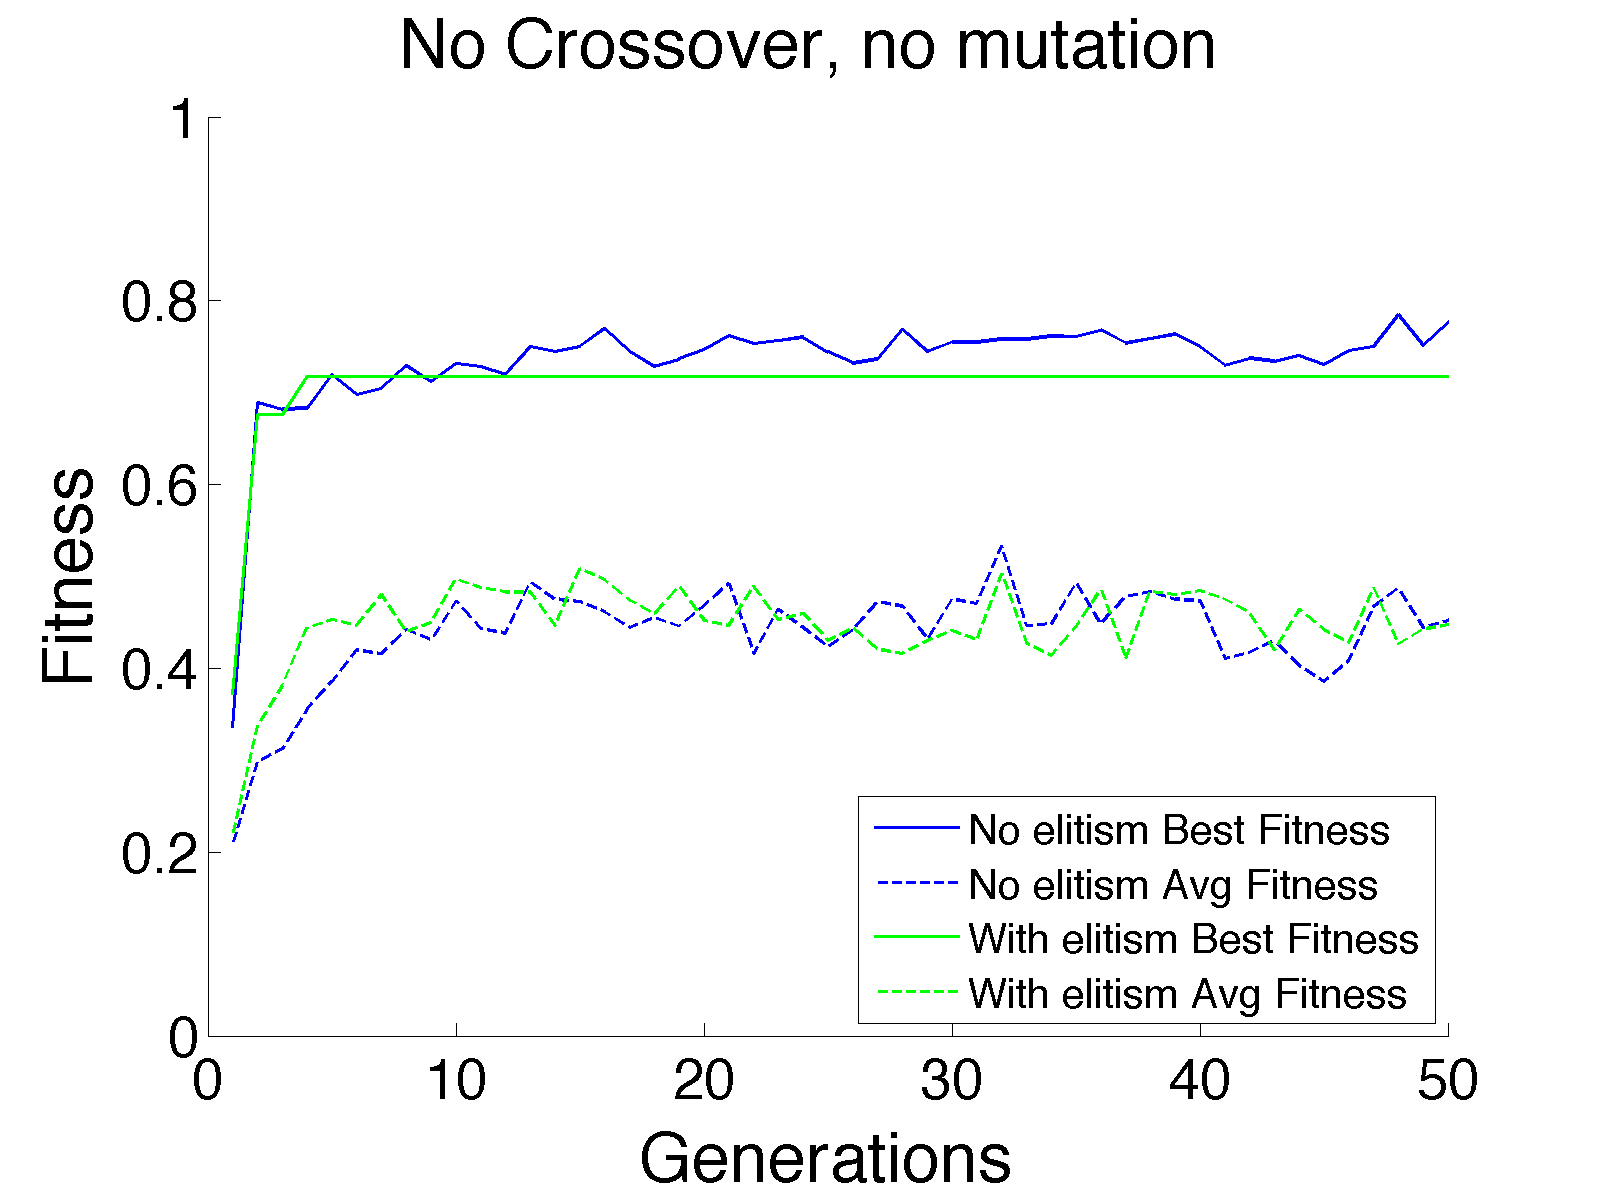
\includegraphics[width=0.6\textwidth,height=0.2\textheight]{figures/fitness0mut0cross.png}
  \caption{Best and average fitness curves with and without elitism with no crossover and no mutation}
  \label{fig:fig1}  
\end{figure}

\begin{figure}[H]
 \centering
  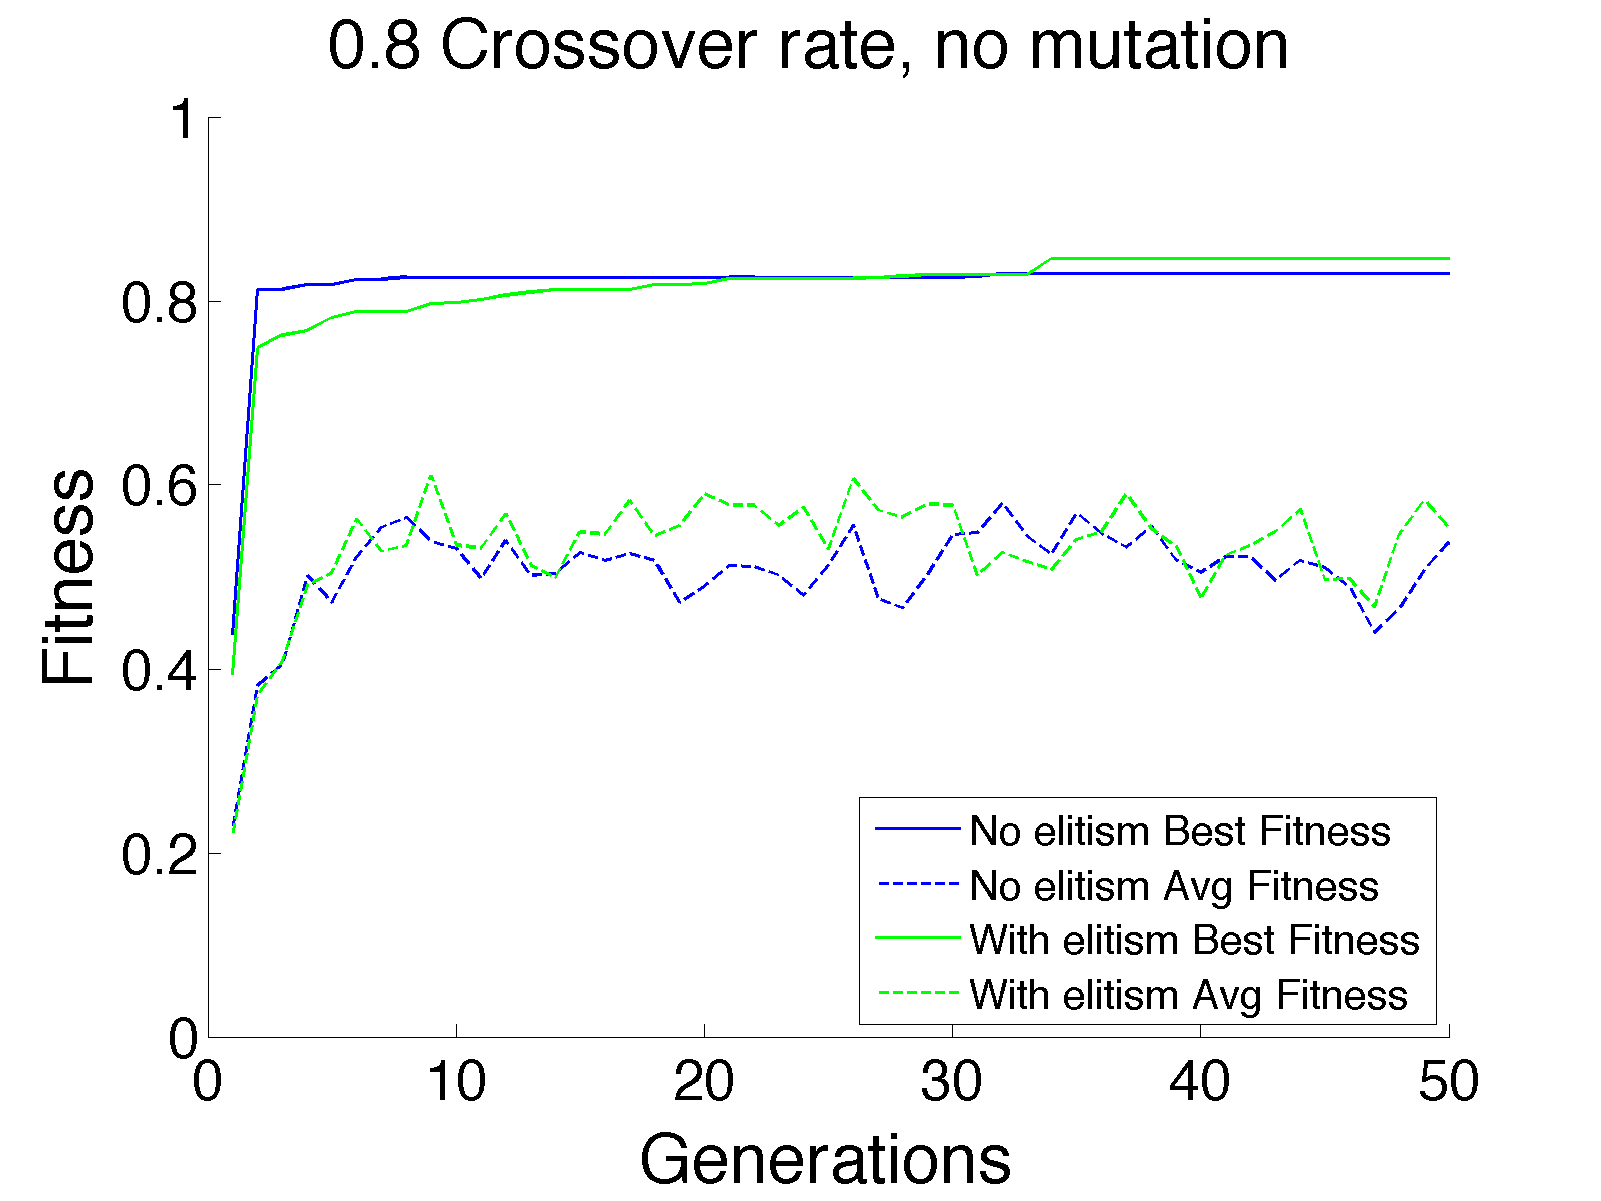
\includegraphics[width=0.6\textwidth,height=0.2\textheight]{figures/fitness0mut08cross.png}
  \caption{Best and average fitness curves with and without elitism with a 0.08 crossover rate and no mutation}
  \label{fig:fig2}  
\end{figure}

\begin{figure}[H]
 \centering
  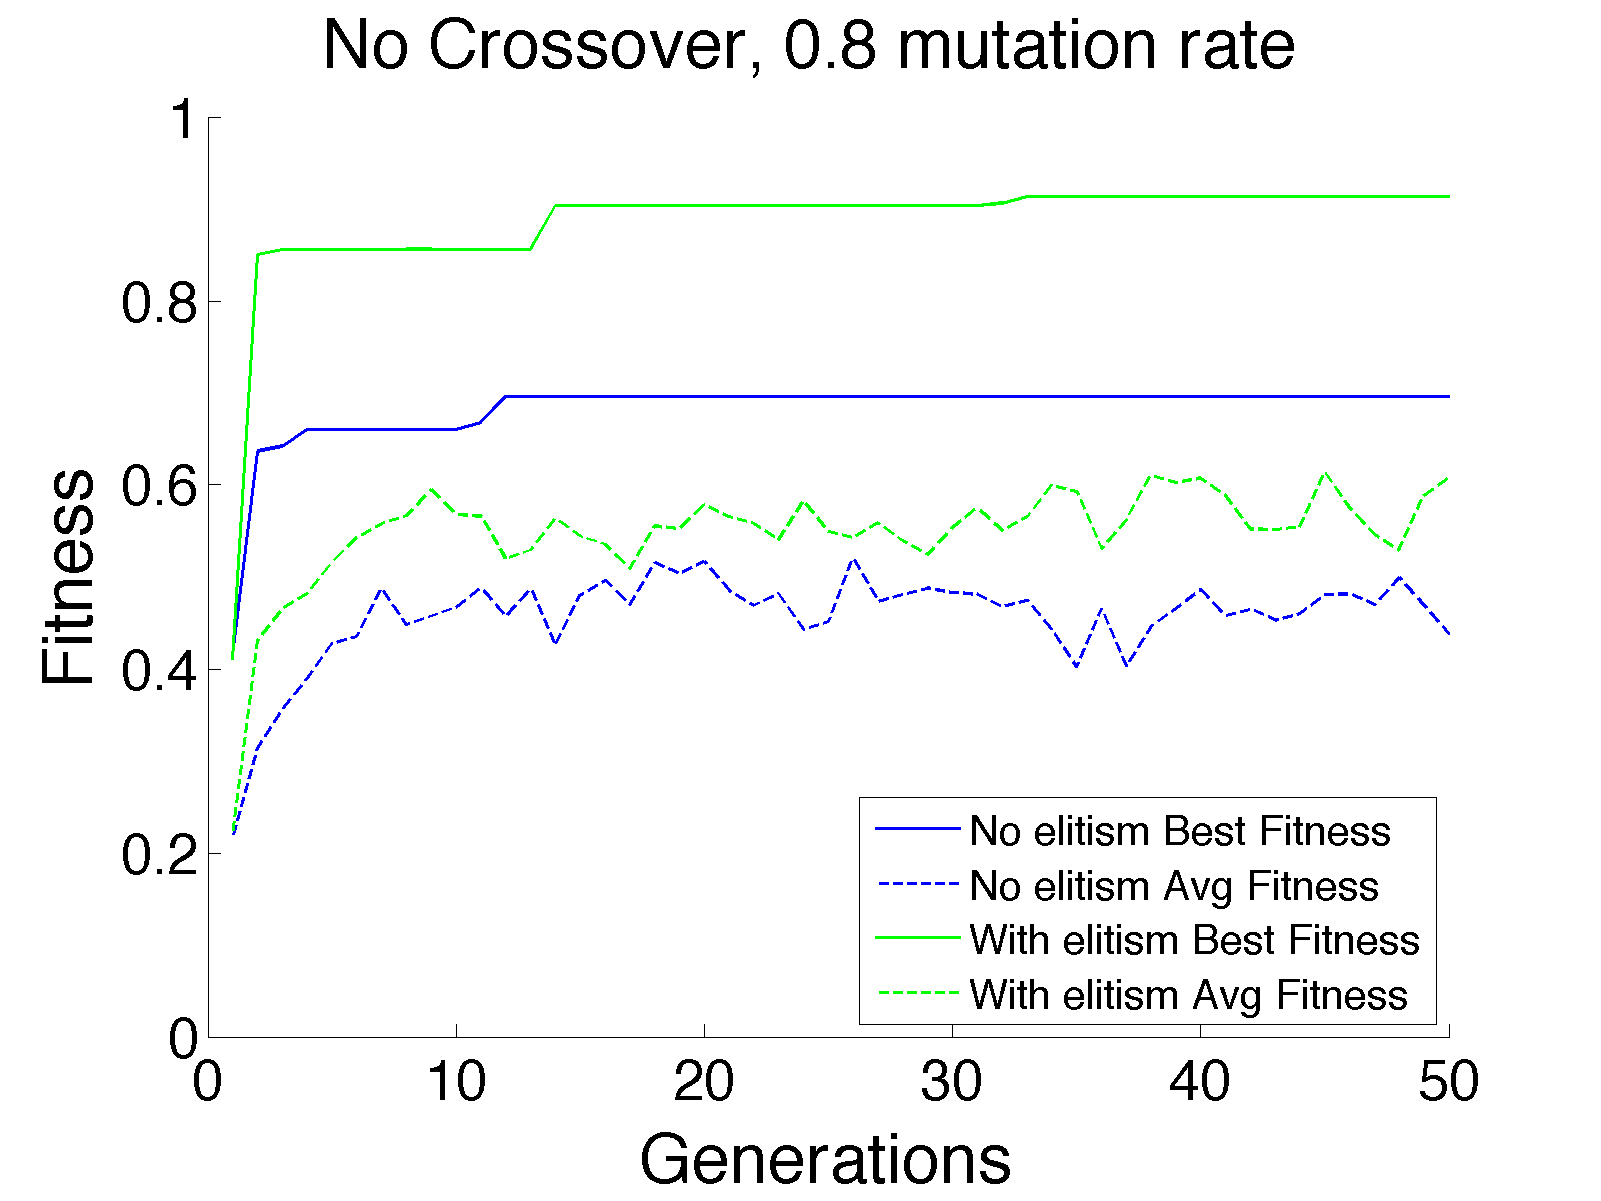
\includegraphics[width=0.6\textwidth,height=0.2\textheight]{figures/fitness08mut0cross.png}
  \caption{Best and average fitness curves with and without elitism with no crossover and a 0.08 mutation rate}
  \label{fig:fig3}  
\end{figure}

\begin{figure}[H]
 \centering
  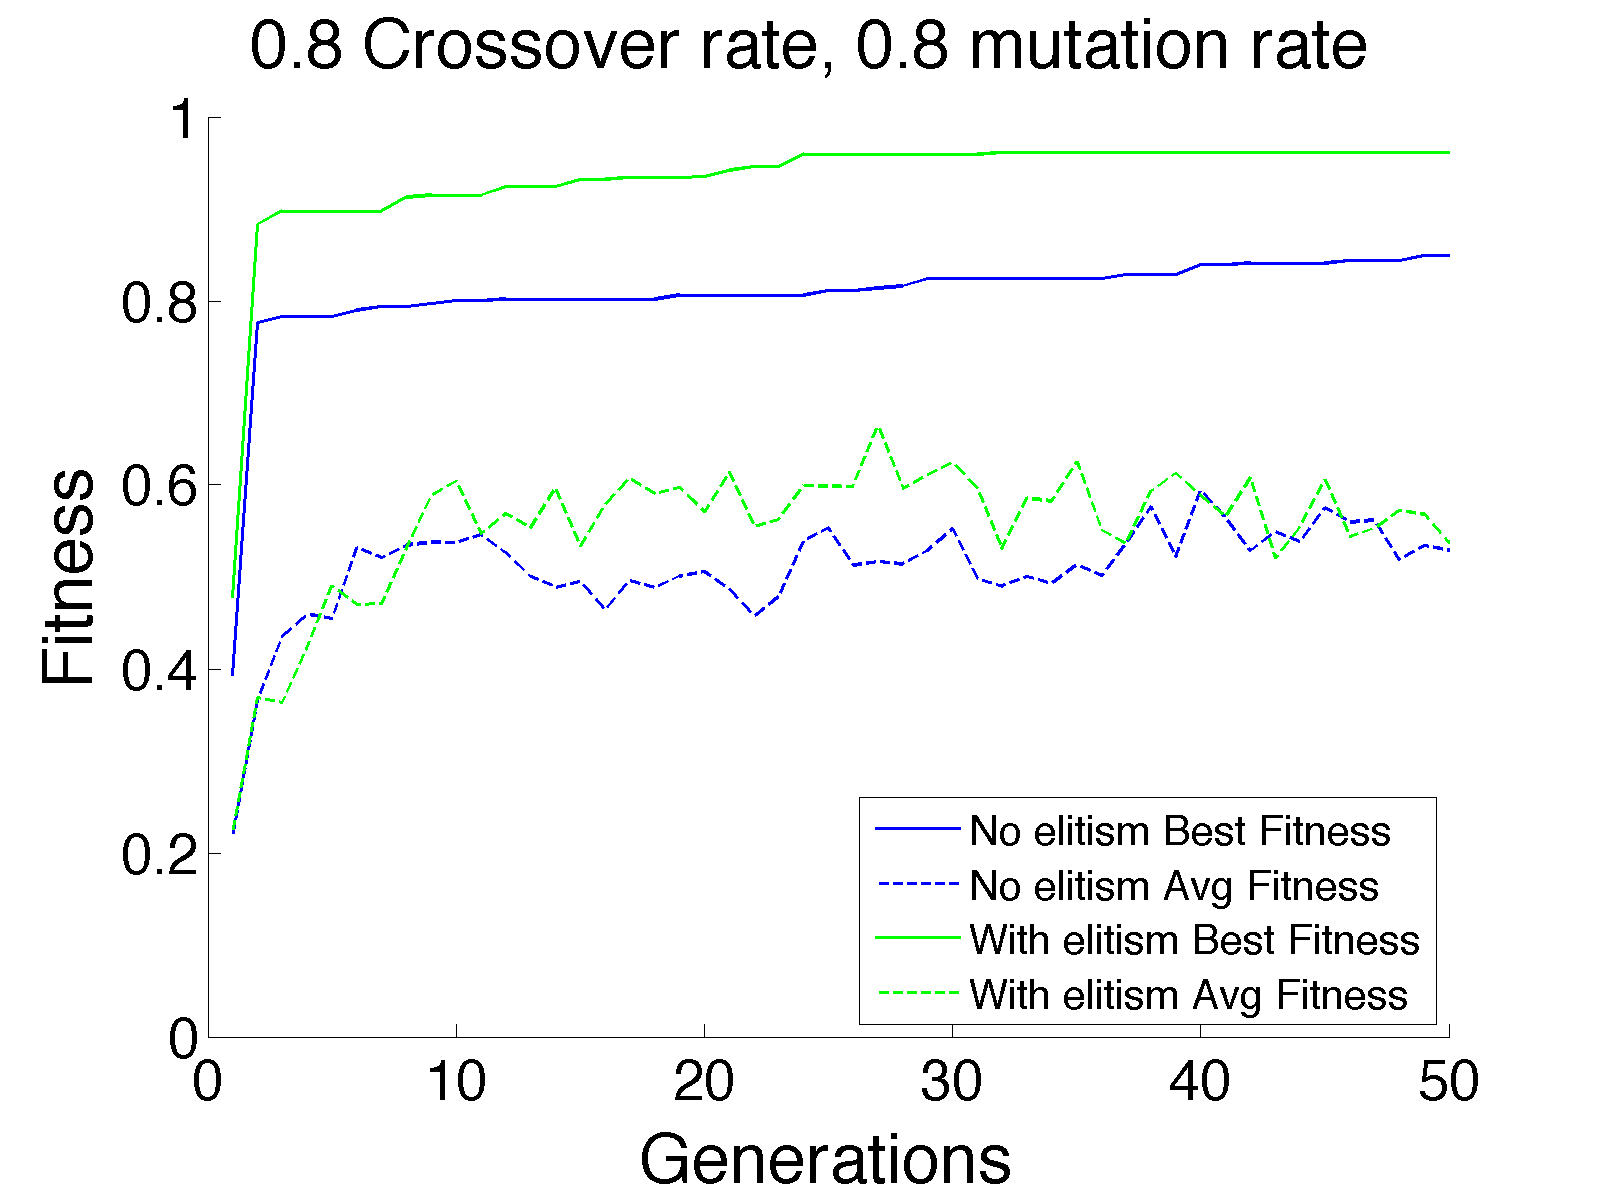
\includegraphics[width=0.6\textwidth,height=0.2\textheight]{figures/fitness08mut08cross.png}
  \caption{Best and average fitness curves with and without elitism with a 0.08 crossover rate and a 0.08 mutation rate}
  \label{fig:fig4}  
\end{figure}
\section{Conclusion}

\bibliographystyle{abbrv}
\bibliography{finalProj_report}
\end{document}


